\section{Durchführung}
\label{sec:Durchführung}

\subsection{Aufbau}
Der Aufbau mit Schaltplanskizze ist in Abbildung \ref{fig:aufbau} zu sehen.
\begin{figure}
    \centering
    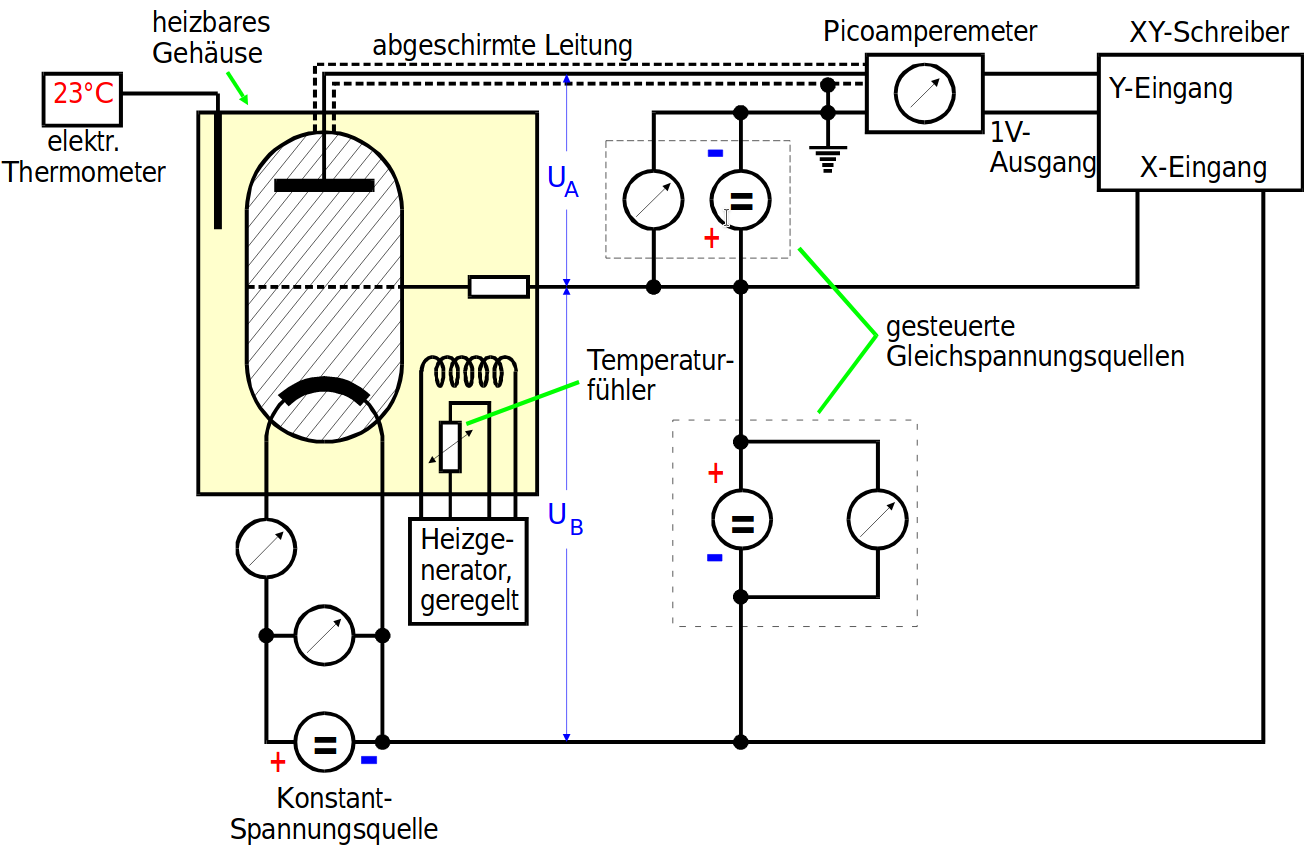
\includegraphics[width=\textwidth]{content/data/aufbau.png}
    \caption{Der Versuchsaufbau mit Schaltplanskizze. Quelle ist die Anleitung zum Versuch \cite[10]{anleitung}.}
    \label{fig:aufbau}
\end{figure}
Da kein XY-Schreiber zur Verfügung stand, konnten die Messwerte nur analog vom Picoampermeter abgelesen werden.
Der sonstige Aufbau entspricht der Abbildung.
Im linken Teil der Abbildung ist die Franck-Hertz Apparatur zu sehen.
Diese besteht aus einer evakuierten Röhre, in welche ein Tropfen Quecksilber gegeben wird.
Dieser verdampft und verteilt sich gleichmäßig in dem Gefäß.
In der Röhre sind zudem ein Glühdraht zur Erzeugung von Elektronen, eine Beschleunigungselektrode, bestehend aus einem Gitter und eine Auffängerelektrode zu finde.
\\
An Auffängerelektrode ist ein Piccoampermeter angeschlossen.
An dem Glühdraht liegt eine konstante Spannung zur Erzeugung der Elektronen an.
Zwischen dem Glühdraht und der Beschleunigungselektrode lässt sich zudem eine varibale Spannung $U_\text{B}$ anlegen.
Zudem lässt scih zwischen Auffängerelektrode und Beschleunigungselektrode eine Spannung $U_\text{A}$ anlegen.
\\\\
Die evakuierte Röhre befindet sich, wie in der Abbildung zu sehen ist, in einem abgeschlossenen Gehäuse.
In diesem Gehäuse ist eine Heizspule, mit der die Temperatur des Gehäuses und somit auch die Temperatur der Röhre verändert werden kann.
Zur Kontrolle der Temperatur befindet sich ein Thermometer im inneren des Gehäuses.
Durch die Änderung der Temperatur lässt sich der Gasdruck des Quecksilbergases beliebig variieren.

\subsection{Messung bei Raumtemperatur}
Der erste Teil des Versuchs wird bei Raumtemperatur durchgeführt, die Heizspule wird also nicht eingeschaltet.
Nun wird die Spannung $U_\text{B}$ zwischen Glühdraht und Beschleunigungselektrode auf eine konstanten Wert von $\SI{11}{\V}$ gebracht.
Die Spannung $U_\text{A}$ wird nun von $\SI{0}{\V}$ in $\SI{0.5}{\V}$-Schritten erhöht, bis kein Strom mehr an der Auffängerelektrode zu messen ist.
Dabei wird nach jedem Schritt der zuvor genannte Strom $I_\text{A}$, welcher am Picoampermeter angezeigt wird, notiert.

\subsection{Messung bei $\SI{140}{\celsius}$}
Im zweiten Teil des Versuchs wird die Heizspule eingeschaltet.
Mit dieser wird die Temperatur im Gehäuse auf $\SI{140}{\celsius}$ geregelt und so konstant wie möglich auf diesem Wert gehalten.
Die Spannung $U_\text{B}$ wird wieder konstant auf $\SI{11}{\V}$ gehalten.
Nun wird allerdings die Spannung $U_\text{A}$ von $\SI{0}{\V}$ in $\SI{0.25}{\V}$-Schritten erhöht.
Die Spannung wird wieder solange erhöht bis kein Stro mehr an der Auffängerelektrode zu messen ist.
Bei jedem Schritt wird wie zuvor auch der Strom, welcher am Picoampermeter angezeigt wird notiert.

\subsection{Messung der Franck-Hertz-Kurven bei $\SI{180}{\celsius}$}
Zur messung der Franck-Hertz-Kurven wird die Temperatur weiter auf $\SI{180}{\celsius}$ erhöht.
Die Spannung $U_\text{A}$ wird auf einem konstanten Wert von $\SI{1}{\V}$ gehalten.
Um nun den Verlauf der Franck-Hertz-Kurven zu messen wird die Spannung $U_\text{B}$ von $\SI{0}{\V}$ auf $\SI{60}{\V}$ erhöht.
Dabei wird die $U_\text{B}$ in $\SI{1}{\V}$-Schritten erhöht, bei jedem Schritt wird der Strom $I_\text{A}$ notiert.
